\documentclass[border=4pt]{standalone}
\usepackage{amsmath,amssymb}
\usepackage{tikz}
\usetikzlibrary{arrows.meta,positioning,decorations.pathreplacing,calc}
\definecolor{cfg}{HTML}{2E7D46}\definecolor{mcfb}{HTML}{2166AC}\definecolor{negr}{HTML}{B03A2E}
\definecolor{inkc}{HTML}{1B1B1B}\definecolor{gy}{HTML}{6B7280}
\begin{document}
\hyphenpenalty=10000\exhyphenpenalty=10000
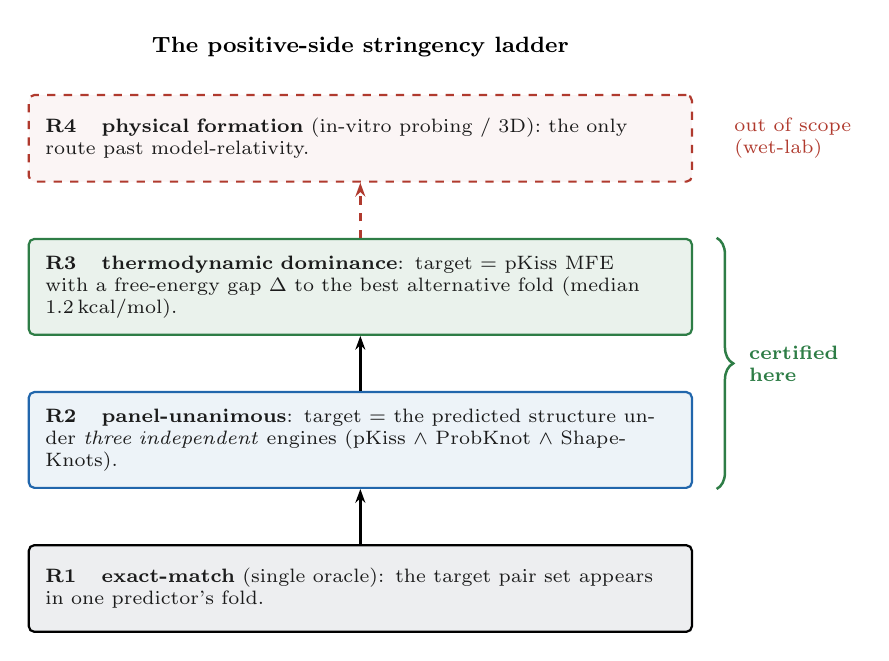
\begin{tikzpicture}[
  >={Stealth[length=5pt,width=3.6pt]},
  r/.style={draw, line width=0.8pt, rounded corners=2pt, align=left, inner sep=6pt, text=inkc,
            font=\scriptsize, text width=80mm, minimum height=11mm},
  up/.style={->, line width=1pt}, font=\scriptsize]

% vertical, left-aligned stack; stringency increases upward
\node[r, fill=gy!12] (r1) {\textbf{R1\quad exact-match} (single oracle): the target pair set appears in one predictor's fold.};
\node[r, draw=mcfb, fill=mcfb!8, above=7mm of r1] (r2) {\textbf{R2\quad panel-unanimous}: target $=$ the predicted structure under \emph{three independent} engines (pKiss $\wedge$ ProbKnot $\wedge$ ShapeKnots).};
\node[r, draw=cfg, fill=cfg!10, above=7mm of r2] (r3) {\textbf{R3\quad thermodynamic dominance}: target $=$ pKiss MFE with a free-energy gap $\Delta$ to the best alternative fold (median $1.2$\,kcal/mol).};
\node[r, draw=negr, dashed, fill=negr!5, above=7mm of r3] (r4) {\textbf{R4\quad physical formation} (in-vitro probing / 3D): the only route past model-relativity.};

\draw[up] (r1) -- (r2);
\draw[up] (r2) -- (r3);
\draw[up, dashed, draw=negr] (r3) -- (r4);

% right-side brace spanning the two certified rungs (R2..R3)
\draw[decorate, decoration={brace, amplitude=6pt}, cfg, line width=0.9pt]
  ($(r3.north east)+(3mm,0)$) -- ($(r2.south east)+(3mm,0)$)
  node[midway, right=8pt, text=cfg, align=left, font=\scriptsize]{\textbf{certified}\\\textbf{here}};
\node[right=4mm of r4.east, text=negr, align=left, font=\scriptsize] {out of scope\\(wet-lab)};

\node[above=3.5mm of r4, font=\footnotesize\bfseries] {The positive-side stringency ladder};
\end{tikzpicture}
\end{document}
